\placelogofalse
\begin{frame}{Basis Functions: FEM Solution Structure}
\begin{columns}
\column{0.58\linewidth}

  $$
    -\Delta u = f \text{ in } \Omega
  $$

\begin{outline}
  \1 Approximate continuous solution to strong form
  \1 Construct solution peicewise
  \2 Basis functions live on element nodes
  \2 Overlap in the elements
  \1 Solution is are weights for basis functions
  \1 Interpolation over mesh for solution
\end{outline}

\column{0.38\linewidth}
\begin{center}
\centering
%\shadowimage[width=2.5cm]{example_1.png}
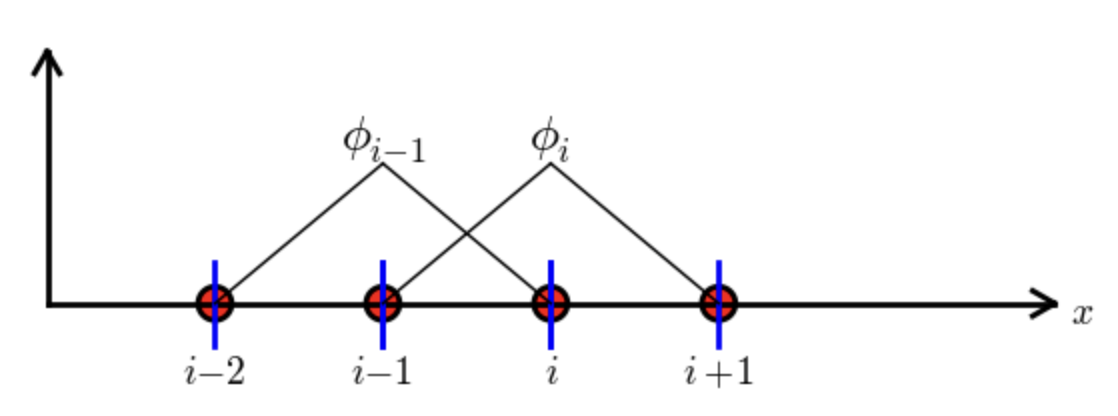
\includegraphics[width=\linewidth]{assets/hat_basis.png}

\vspace{0.5cm}

\shadowimage[width=\linewidth]{assets/base_functions_overlap.png}

% [trim={left bottom right top},clip]
%
\includegraphics[width=8.5cm, page=3, trim={0 9cm 14cm 0cm},clip]{assets/vec_db_figs.pdf}
\end{center}
\end{columns}
\end{frame}
\placelogotrue
